% !TEX root = ../Dissertation.tex
%===================================================================================================

\chapter{Discussion}

Type 1 diabetes is believed to be due, in part, to a breakdown in central tolerance of T cells in the thymus.
Our studies, and others, have correlated a significant increase in thymic B cells in NOD mice, with respect to diabetes-resistant murine strains, with T1D progression to the $\beta$ cell destruction phase.
The origin and role of these B cells are not known, but they might possibly be involved in the breakdown of central tolerance.
Due to the strong correlation between thymic B cell numbers and T1D susceptibility, it is important to establish how intrathymic abnormalities occur in NOD mice.
This project aims to investigate more fully the potential intrathymic development of B cells.

Through this project, it has been confirmed that B cells are increased in the NOD mouse thymus with respect to B6 control mice, and that this increase is age-related.
In terms of potential intrathymic development, it has been shown that the thymus contains B cell development transcription factors and, therefore, could be conducive to B cell development.
Also, pro and pre B cells are present in the thymus of NOD mice, though the population frequency appears to be dependent on the presence of a mature B cell.
Further to this, there is evidence of active B cell receptor rearrangement in the thymus, indicative of active B cell development.
However, the progenitor from which thymic B cells are originating from is less clear. 
Whilst BLPs are present in both NOD and B6 mouse thymi, they are significantly decreased in the NOD mouse compared to B6 mouse suggesting an alternative progenitor for thymic B cells, at least in the NOD mouse.

Also, further to these findings, there were some interesting results which suggested the presence of a cell in the thymus expressing markers of both T and B cells, and in fact a small population expressing both a B and T cell receptor.
These could provide an alternative mechanism for B cell development through re-differentiation of T cells.


\section{There is an age-related increase in thymic B cells in the NOD mouse}

The results showing an age-related increase in thymic B cells in the NOD mouse compared to the B6 control mouse suggests there may be a correlation between thymic B cells and T1D progression.
T1D onset occurs with initial priming of T cells between 3-5 weeks of age. 
At this point there is minimal responsiveness of T cells to T1D antigens and the population of B cells in the NOD thymus is not increased compared to control B6 mice.
At 5 weeks of age, the islets start to become infiltrated with immune cells and by 9 weeks, CTL mediated $\beta$ cell destruction is initiated and progresses to destroy the majority of $\beta$ cells.
In terms of thymic B cell numbers, B cells are significantly increased at 9 weeks of age in NOD mice compared to B6, and further increased by 12 weeks.


T cell development and education occurs within the thymus, in particular the first step of T cell tolerisation, negative selection.
This is where autoreactive T cells are purged from the repertoire to prevent potential autoimmunity \citep{Hogquist2005}.
T1D is believed to be due to a breakdown in tolerance and, therefore, it may be that B cells found in the thymus of NOD mice may be contributing to this process.
There is evidence that B cells are able to contribute to the process of negative selection, as shown by \citet{Frommer2010} and \citet{Yamano2015}.
\citet{Yamano2015} have demonstrated that B cells found in the thymus, but not the periphery, are able to express AIRE, similar to mTECS which classically mediate negative selection.
Using AIRE-reporter mice, donor splenic B cells were transferred into recipient mice then the thymi of the recipient mice were analysed one week after transfer.
It was observed that there were AIRE expressing donor cells in the thymus of the recipient mice.
This suggests that there may be something in the thymic environment which is causing B cells to express AIRE upon entering the thymus.
MHC class II, also important for mediation of negative selection, was also upregulated on the immigrating thymic B cells.
Meanwhile, \citet{Frommer2010} utilised a mouse that specifically expressed myelin oligodendrocyte glycoprotein (MOG) on MHC class II of all B cells, including thymic B cells (B\textsuperscript{MOG} mice). 
These mice were then crossed with a transgenic mouse with has a T cell repertoire specific for MOG (2D2 mice).
Interestingly, in the resulting mice (B\textsuperscript{MOG}/2D2 mice), the frequency of CD4\textsuperscript{+} T cells was significantly reduced in the thymus and periphery, compared to 2D2 mouse controls.
After ruling out the possibility of mTECs and other APCs in the thymus expressing the MOG antigen and, therefore, contributing to the negative selection of the MOG specific T cells, it was shown that the deletion of MOG specific T cells in the thymus was as a result of MOG expression on MHC Class II of B cells. 

In the above studies, non-autoimmune prone mice were utilised in which the autoimmune process was inititated by inducing the inappropriate expression of host antigens and biasing the T cell repertoire to recognise these antigens.
In these cases, the role of the B cells in the thymus appeared to be beneficial to the host in the tolerance induction in developing T cells.
However, it is plausable that in autoimmune prone mice, such as the NOD mouse, the B cells may, in fact, be detrimental to the negative selection of T cells.
%Supposing thymic B cells are having an affect on negative selection, it is not known if their contribution is useful in aiding removal of autoreactive developing T cells, or a hindrance to their deletion.
It could be that thymic B cells are a driving force in the breakdown of negative selection, and that the increase in thymic B cells seen in the NOD thymus, compared to control B6 mice, is linked to an increasing breakdown in negative selection.
On the other hand, as previous literature suggests that the negative selection provided by thymic B cells is beneficial in T cell education, it may be that increased thymic B cells are a consequence of the disease process, such that their development is triggered to help with an increasing population of developing autoreactive T cells.

Investigation into the role of thymic B cells was outside the remit of this project but it remains a fundamental area that neccessitates further research in the future.



\section{B cells are developing intrathymically}

\subsubsection{Thymic pro and pre B cell presence}
The main hypotheses for the origins of thymic B cells are (a) intrathymic development from progenitors, or (b) migration of B cells from the bone marrow to the thymus.
The general consensus is that B cells are developing within the thymus with very little contribution from the circulation.
Experiments involving parabiotic congenic mice (where two congenic mice share the same blood system) showed that of the thymic B cells, the majority were of the endogenous phenotype, not the parabiotic partner. 
This gave the impression that the presence of thymic B cells have more to do with the signals within the thymus itself, rather than alteration in the circulation pattern of B cells \citep{Perera2013}.
Similarly, \citet{Akashi2000} found that the majority of thymic B cells were of host origin.
To investigate this, donor adult (Ly5.1 x Ly5.2)F1 mouse splenic B cells were injected into Ly5.1 recipient mice.
The percentages of B cells of donor- and recipient-derived B cells were then evaluated in the thymus and periphery of the recipient mice.
In the periphery, approximately 5-7\% of B cells were of donor origin, compared to approximately 0.06\% of thymic B cells of donor origin.
This gives the impression that thymic B cells are mainly of host origin, rather than as a result of B cells entering the thymus from the circulation. 

This project aimed to further investigate this intrathymic development and the evidence from the data shown agrees with the hypothesis of intrathymic B cell development.

Firstly, pro and pre B cells were investigated in the thymus of both NOD and B6 mice and shown to be present. 
This is similar to the findings of both \citet{Hashimoto2002}, who showed presence of pro B cells and a smaller population of pre B cells in the thymus of BALB/cJ mice, and \citet{Akashi2000}, who both showed presence of pro and pre B cells in the thymus of B6 mice.
It would seem, therefore, that the ability of B cells to develop in the thymus, at least to the pro B cell stage, is common for both diabetes-prone and diabetes-resistant strains of mice.

\citet{Hashimoto2002} also showed an interesting finding that in BALB/cJ mice, there was an accumulation of pro B cells in the thymus that were inefficient at maturing to the pre B cell stage and beyond.
Through foetal thymic organ culture (FTOC), it was hypothesised that the thymic environment renders B cell progenitors hyporesponsive to lymphopoietic signals, such as IL-7.
This was shown by seeding lobes with B cell progenitors from the bone marrow, then harvesting the cells at both 2 and 7 days post seeding.
Following harvest, cells were cultured on S17 bone marrow stromal cell lines with B cell permissive conditions and it was shown that only those harvested at the 2 day time point were able to produce B cells, whereas the 7 day time point cells were not.
Il-7 is important for B cell development \citep{Corfe2012}. \citet{Hashimoto2002} showed that B cell progenitors from FTOC showed a decreased response to IL-7 compared to the same B cell progenitors taken directly from the bone marrow.
However, these data were acquired using in vitro approaches therefore it is not known whether this is applicable to the processes in vivo.

The presence of pro and pre B cells in the NOD thymus suggests that B cells may be developing there as they are two fundamental stages of normal B cell development (see \cref{Bcelldev}).
The findings by \citet{Hashimoto2002} could also suggest a potential mechanism by which B cells are increased in the NOD thymus compared to the control B6 mouse thymus, in that the NOD thymic environment may be less effective at dampening B cell progenitor responsed to lymphopoietic signals, such as IL-7.

Interestingly, it appears that the frequency of the thymic pro B cell population is dependent on whether or not mature B cells are present.
That is, in NOD KO mice, the frequency of thymic pro B cells was significantly reduced compared to in both NOD and B6 mouse thymi.
%This result was not expected and begs the question as to how to investigate this further.
Some potential roles of a mature B cell include the following:
\begin{itemize}
\item A mature B cell may be helping with the recruitment of B cell progenitors from the bone marrow to the thymus
\item A mature B cell may provide a survival factor for B cell progenitors within the thymus so that they survive to be able to develop
\item Mature B cell presence may kick start the process of B cell transcription factor expression within the thymus, so that the thymus can provide an environment conducive to B cell development
\item A mature B cell may provide a survival factor for newly developed B cells so that once they have developed, they are able to survive.
\end{itemize}

A potential mechanism for investigating the role of mature B cells on the thymic pro B cell population would be to transfer mature B cells from a B cell sufficient NOD mouse into the NOD KO mouse to see if these donor B cells can have an effect on the thymic pro B cell population.
However, a pilot study of this method was attempted and showed that the donor B cells did not survive to 11 days post transfer.

A similar approach to infuse mature B cells into NOD KO mice has also been attempted by \citet{Serreze1998} where mature splenic B cells were transferred into NOD KO recipient mice. 
A similar finding was observed in that the B cells disappeared between 6 and 11 days post transfer.
\citet{Serreze1998} showed that this disappearance was due to CTL destruction of the donor B cells, presumably due to the lack of B cell presence during endogenous T cell development, therefore, the T cells would never have been tolerised to B cells.
%However, it is not known if this is also the case in the transfer experiment shown in this project.
It is not known if CTL mediated B cell destruction was also occuring in the transfer utilising thymic B cells (rather than splenic), or whether it was a different mechanism causing their disappearance. 
However, given the fact that these B cells disappear following transfer, it suggests that this approach may not be appropriate for determining the effect of mature B cells on the thymic pro B cell population.
For mature B cells to exert their effects on the thymic pro B cells, they may need to be present for longer than the period they are detectable in the recipient NOD KO mice, therefore, an alternative approach must be explored.
%If CTL mediated destruction is the cause, it would be of interest to know where this killing was taking place. 
%For example, B cells were seen in both the spleen and thymus at the 7 day post transfer time point.
%Therefore, unless B cells that have reached these tissues leave again and are then destroyed, it suggests that CTL activity may be happening within the thymus and spleen. 

%The fact the mature donor NOD B cells disappear following transfer into the NOD KO mice means that the approach may not be appropriate to determine the effects of mature B cells on thymic pro B cell populations means that an alternative approach must be found.
\citet{Serreze1998} continued investigations by irradiating recipient mice then transplanting NOD KO bone marrow supplemented with NOD B cells.
This results in endogenous effector immune cells developing in the presence of B cells and should avoid the T cell destruction of donor B cells.
This could, therefore, be a way forward to investigate the effect of B cells on the population of pro B cells in the NOD KO thymus.
By adding purified mature B cells, it would be interesting to see if this was sufficient to increase pro B cell frequency in the KO thymus.
Following this, it would also be of interest to try transplanting KO bone marrow supplemented with B6 B cells to see if it is a characteristic of a NOD B cell that can increase thymic pro B cells.
However, transfer of B6 B cells into NOD mice would result in rejection therefore it would be necessary to use mice such as B6.H-2g7 (\citep{Gonzalez1997}) which express NOD MHC and would not be rejected. This then carries the caveat of the MHC being of NOD origin and may mean that the differential effects of a NOD B cell and a B6 B cell on the thymic pro B cell population may be hidden if their action has anything to do with MHC.
Furthermore, it is not known whether the mature B cell needs to be of splenic or thymic origin, therefore, these experiments could also test this by separately transferring bone marrow supplemented with B cells from both tissues.

\subsubsection{BcR rearrangement in the thymus}


For pro B cells to progress to the pre B cell stage, the IgM heavy chain must be rearranged.
Therefore, it was wondered whether the thymus is able to support this developmental step.
To tackle this question, RAG expression within the thymic CD19\textsuperscript{+} cells was assessed in NOD mice.
It was seen that there are populations of CD19\textsuperscript{+}RAG\textsuperscript{high}, CD19\textsuperscript{+}RAG\textsuperscript{low} and CD19\textsuperscript{+}RAG\textsuperscript{-} cells in the NOD thymus.
The RAG\textsuperscript{high} cells are very likely developing there within the thymus as this very bright signal was equivalent to that seen in actively developing T cells in the thymus and actively developing B cells in the bone marrow.
This gives the impression that RAG is being actively transcribed in CD19\textsuperscript{+} cells in the thymus, indicating active BcR rearrangement and B cell development.
In addition, if B cells were rearranging their receptors in the bone marrow and then migrating to the thymus, the GFP expression seen in the thymic B cells would be lower due to the kinetics of GFP expression.
Evidence for this is seen when screening the blood of GFP\textsuperscript{+} transgenic mice to see if they are indeed GFP\textsuperscript{+}. In this case, no GFP\textsuperscript{high} cells are seen in the blood of the mice suggesting that GFP expression is decreased following release from the bone marrow. Therefore, GFP\textsuperscript{high} B cell in the thymus is more likely to be due to active development there, rather than left over GFP from rearrangement in the bone marrow (E.A. Green, personal communication).

These RAG expressing CD19\textsuperscript{+} cells were looked for in NOD-RAG-GFP mice of 4, 7 and 11 weeks of age and interestingly, the CD19\textsuperscript{+}RAG\textsuperscript{high} population frequency didn't change, whereas the CD19\textsuperscript{+}RAG\textsuperscript{low} frequency decreased significantly.
This gives the impression that as mice age, there are less newly developed B cells in the thymus, potentially as a result of decreased development.
This decrease suggests that the development of B cells within the thymus may be restricted to younger mice and that that intrathymic B cell development may be deactivated at a certain time point in the disease process.
However, it may be that more newly developed B cells are leaving the thymus in older mice compared to younger ones so that the population of newly developed B cells within the thymus is decreased.

If the decrease in CD19\textsuperscript{+}RAG\textsuperscript{low} cells is due to a decrease in development, this may be due to the fact that within the thymus there are multiple different niches harbouring different types of cells.
For example, the proliferation of DN thymocytes depends on the availability of stromal niches within the thymus and this is capable, therefore, of regulating the thymus size \citep{Prockop2004}.
It may be that within the thymus, there is a niche that is more capable of allowing B cell development than others.
Further to this, it may be that this niche is more prevalent in mice of NOD background compared to non diabetic controls.
If this is the case, downregulation of B cell development may occur as a result of the thymic B cell niche becoming full and competition may prevent the development of more B cells.
Further to this, thymi undergo atrophy with age, therefore, a thymus which is decreasing in size would have less space available for cells, including B cells, to reside in, so it may be that with increasing age, B cell development is decreased.
Thymic atrophy is believed to be accelerated in the NOD mouse.
As shown by \citet{Ferreira2014}, thymic involution and loss of thymic architecture is seen by 9 months of age in the NOD mouse, whereas equivalent thymic degradation in the B6 mouse is not seen until 15 months of age.

On the other hand, if newly developed B cells are leaving the thymus and travelling elsewhere, it may be that the thymus is acting like the bone marrow, harbouring B cell development then allowing their release to mature in a different tissue, such as the spleen.
In this regard, it would be interesting to know if thymic egressed B cells contribute to breakdown in peripheral tolerance of T cells to $\beta$ cells. 

Neither of these suggestions account for the overall picture of an increase in B cells in the NOD mouse thymus compared to the B6 mouse thymus.
It does, however, suggest that the increased population of thymic B cells may not be directly linked to the rate of B cell development, but more to proliferation of developed B cells.

By understanding the kinetics of intrathymic B cell development, and the potential impact of thymic B cells on the normal functioning of the thymus, this could aid in the design of potential therapeutics.
This understanding could ellucidate a specific disease time point to target with a therapeutic agent, in order to have the greatest impact on limiting disease progression.


\subsubsection{BLPs are present in the NOD thymus}

As mentioned in \cref{subsec:Bcelldevelopment}, the commitment of progenitors to the B cell lineage is thought to occur at the Sca-1\textsuperscript{low}c-kit\textsuperscript{low}Flt3\textsuperscript{+}IL-7R$\alpha$\textsuperscript{+}Ly6D\textsuperscript{+} BLP stage (\cref{Bcelldev}, red cell labelled `BLP').
Therefore, it was wondered whether these BLPs would be present in the NOD thymus and, if so, if they are increased in the NOD mouse compared to the B6 mouse.
When looking for potential TSPs, cells with the correct markers to allow homing were considered \citep{Zlotoff2011}, therefore, it may be that marker expression in the bone marrow is abherrent on B cell progenitors, resulting in an excess of B cell precursors being able to migrate to the thymus alongside T cell progenitors.
For example, due to their fundamental role in allowing thymic settling of progenitors, it would be of interest to see how the levels of Flt3, CCR7 and CCR9 expression compared between bone marrow BLPs and BLPs found in the thymus \citep{Zlotoff2011, Zlotoff2010}.
It may be that some express excess levels of these markers which allow B cell progenitors to migrate to the thymus along with TSPs.

It was interesting when investigating the presence of BLPs that the frequency of BLPs in the Sca-1\textsuperscript{low}c-kit\textsuperscript{low}Flt3\textsuperscript{+}IL-7R$\alpha$\textsuperscript{+} population in the thymus of the NOD mouse, was significantly decreased compared to the B6.
This was surprising due to the increased population of B cells seen in the NOD thymus compared to that of the B6.

However, before any assumptions can be made on this data, it is first necessary to consider the model of B cell development from BLPs.
For example:
\begin{itemize}
\item Are BLPs the sole progenitor for B cell development? There is evidence to suggest that this is a progenitor that is restricted to the B cell lineage \citep{Inlay2009}, however, it is not clear if this is the only progenitor capable of differentiating into a B cell.
\item Is the B cell developmental pathway the same in the thymus as the bone marrow? The B cell development pathway in the bone marrow has been investigated extensively \citep{Welinder2011}, however, the pathway in the thymus is much less well understood, therefore, whether the bone marrow development pathway can be applied to the thymus is not known. 
\end{itemize}

In order to help determine the answers to the questions above, it would be necessary to carry out further experiments.
To determine whether B cells can develop from thymic BLPs, it would be interesting to culture BLPs on thymic stromal cell lines, such as OP9-DL1 cell lines (Notch ligand-expressing, bone marrow derived cell line) which can, to an extent, simulate the thymic environment \citep{Holmes2009}.
It would, therefore, be useful to see if BLPs are able to develop into B cells on cell lines such as these.
It would also be of use to confirm whether the BLPs identified in the thymus in this project are able to differentiate into B cells under the same conditions as those described by \citet{Inlay2009} when characterising the bone marrow-derived BLP.
For this, liquid culture, supplemented with stem cell factor (SCF), Flt3L and IL-7, was used and differentiation of BLPs into B cells was seen.
By replicating these conditions and culturing thymus-derived BLPs, it could suggest whether or not they are able to produce B cells in the way that bone marrow-derived BLPs can.
%This would suggest whether or not the bone marrow BLPs, suggested by the likes of \citet{Inlay2009}, are the same as those identified in the thymus.

It is unlikely that B cell development from BLPs is restricted only to the bone marrow, shown by the presence of BLPs in the B6 thymus.
These may be the origin of the normal, small population of B cells in the B6 thymus.
However, the NOD thymus has a significantly smaller frequency of BLPs in the thymus compared to the B6.
Despite this, NOD mice still have increased thymic B cells suggesting that there are different mechanisms in the NOD mouse which increase thymic B cells that are not present in the B6 mouse.

Interestingly, when comparing NOD and NOD KO thymic BLPs, there was no difference observed in the population frequency.
This means that if a mature B cell is having an effect on the pro B cell population, it's action must be after the formation of the BLP, and prior to the formation of the pro B cell.
For this reason, it would be of interest to investigate stages between these two cells, to see whether they are affected by the presence/absence of mature B cells and to try and pinpoint the time point when mature B cells have their effect.

\subsubsection{Do thymic T cells transition to B cells?}

To understand another potential mechanism for increased thymic B cells, the finding of RAG\textsuperscript{+}CD19\textsuperscript{+}CD4\textsuperscript{+}CD8\textsuperscript{+} cells in the thymus needs to be considered.
It is worth noting that the numbers of mice investigated was relatively small and, therefore, requires further repetitions, along with inclusion of B6 control mice for comparison.
However, assuming that this population is a true, distinct cell population in the thymus of NOD mice, there are a few potential hypotheses relating to these cells.
One in particular is of interest for the increased thymic B cells seen in the NOD mouse.
These cells expressing markers of both T and B cells suggest that there may be an intrathymic, post-CLP stage when developing T and B cells express dual T/B cell markers.
However, if this is the case, it is unlikely that this stage is a normal part of B cell development in the bone marrow due to the lack of RAG\textsuperscript{+}CD19\textsuperscript{+}CD4\textsuperscript{+}CD8\textsuperscript{+} there.
%On the other hand, this process is unlikely to be a normal part of either developmental pathway due to the absence of these cells in the bone marrow (therefore unlikely to be a part of B cell development) and the fact that T cells are committed to the T cell lineage at the DN stage (prior to CD4 and CD8 expression).

Thymic progenitors are normally committed to the T cell lineage at the DN stage, that is, prior to CD4\textsuperscript{+} and CD8\textsuperscript{+} expression.
It is, therefore, worth considering whether RAG\textsuperscript{+}CD19\textsuperscript{+}CD4\textsuperscript{+}CD8\textsuperscript{+}  cells represent developing T cells which are late to commit to the T cell lineage and are retaining some characteristics of B cells (CD19).
On the other hand, they may be cells developing with characteristics of both T and B cells.
This may be possible due to the finding of a small population of cells expressing both a TcR and BcR (IgM\textsuperscript{+}TcR$\beta$\textsuperscript{+}) in the thymus that may be the mature cell for which RAG\textsuperscript{+}CD19\textsuperscript{+}CD4\textsuperscript{+}CD8\textsuperscript{+} cells are the progenitor.

Another possibility which could then contribute to the B cell population in the thymus, is that these cells are the midpoint of a T cell transitioning to a B cell (or vice versa, although this would not account for increasing thymic B cells).
%This would account for there only being a very small population of IgM\textsuperscript{+}TcR$\beta$\textsuperscript{+} cells, and the expression of both T and B cell markers.
This could account for the decreased BLPs in the NOD compared to B6, as B cells developing from T cells would not develop originally from BLPs and could, therefore, provide an alternative `progenitor' to a mature B cell.

To investigate the potential for T cell to B cell (or vice versa) transition, it would be of use to look at the relative levels of B and T cell transcription factors Pax5 and Notch1 in the thymus of NOD mice compared to the thymus of B6 mice.

Maintaining the correct balance of transcription factors is very important for development of lymphocytes. 
For example, as mentioned in \cref{subsec:Bcellgenes}, Pax5 expression is important for repressing T cell lineage commitment through the repression of Notch1 \citep{Souabni2002}.
This was shown by expressing Pax5 in all HSCs and MPPs and it was found that the constitutive expression of Pax5 led to an increase in B cell development, and a simultaneous decrease in T cell development due to Pax5 dependent repression of Notch1.
%It is also thought that T cells only commit to the T cell lineage and lose B cell potential once progenitors arrive in the thymus \citep{Heinzel2007}.
Further to this, deletion of Notch1 led to a loss of developing T cells and an increase in thymic B cells \citep{Feyerabend2009}.
As shown by \citet{Feyerabend2009}, they found that when Notch1 was deleted from progenitor T cells, this was associated with an increase in thymic B cells, some of which arose from the progenitor T cells switching fate from T to B cell lineage.
However, unexpectedly, the majority of these B cells arose from Notch1 sufficient progenitors and, therefore, became B cells as a result of a cell-extrinsic factors acting due to the deletion of Notch1 in progenitor T cells.

That said, Notch1 is not the only important transcription factor that needs to be kept in balance.
As mentioned in \cref{subsec:Tcellgenes}, Gata3 is an important transcription factor for T cell development which requires repression by EBF for B cell development to occur \citep{Banerjee2013}.
\citet{Banerjee2013} showed, through the use of quantitative PCR, that EBF is capable of significantly reducing Gata3 transcription.
This was done by transfecting ebf\textsuperscript{-/-} progenitor cells prior to the pro B cell stage, with EBF and/or Pax5.
Following induction of Pax5 expression, Notch1 transcripts were found to be consistently decreased and EBF expression reduced Gata3 transcript abundance.
This suggests that EBF is also able, to an extent, to control the T/B cell fate decision and, therefore, any abnormality in expression levels may affect the populations of B and T cells in the thymus.
In terms of BLPs identified in this project, when \citet{Banerjee2013} looked into the levels of Gata3 transcripts in these cells they found a robust decrease compared to that seen in all-lymphoid progenitors (ALPs).
This coupled with the lack of T cell lineage cells arising from BLPs suggests that Gata3 may be downregulated when T cell potential is lost.

\citet{Cobaleda2007} have shown that B cells, in the correct conditions, may be able to de-differentiate back to progenitors, and then differentiate into T cells.
To show this, Pax5 was deleted from mature B cells from Ly5.2\textsuperscript{+} donor mice and the B cells were then transferred into recipient Ly5.1\textsuperscript{+} mice.
It was found that 8 weeks after transfer, some of the donor mature B cells had dedifferentiated back to the pro B cell stage, shown by their Ly5.2\textsuperscript{+} pro B cell phenotype.
Also, the recipient mice (that were T cell deficient) showed reconstitution of T cell development in the thymus 8 weeks following transfer of Pax5 deleted B cells.

These data, combined, show the importance of transcription factor balance.
It may be that in the thymus of NOD mice, an imbalance in transcription factor expression causes the increased B cell population.
%A good way to investigate this would be to carry out quantitative PCR of the very important B and T cell transcription factors which appear to be present in the thymus.
%For example, Notch1 and Gata3 would be of interest to compare the abundance of transcripts seen in both NOD and B6 thymi to see if there is any difference between the two strains.
%Also, Pax5 and EBF would be of interest to compare the abundance of transcripts of these seen in the thymus, with the levels seen in the bone marrow to see how they compare.
Given the information on transcription factor balance importance above, it would also be beneficial to compare the relative levels of Notch1 and Pax5, and Gata3 and EBF seen in the thymus of NOD and B6 control mice.
This could indicate any imbalance, unique to the NOD mouse, which could be accounting for the increased thymic B cell population seen in the NOD thymus.
Unfortunately, due to time constraints, quantitative PCR studies to assess the transcription factors above could not be conducted.


In the future, to investigate the potential transitioning of a T cell to a B cell (or vice versa) in the thymus, RAG\textsuperscript{+}CD19\textsuperscript{+}CD4\textsuperscript{+}CD8\textsuperscript{+} cells could be isolated and their final developmental fate determined following incubation with either a stromal cell line (such as OP9-DL1), or more relevantly, a reaggregated thymic organ culture (RTOC).
In this latter approach, developing thymocytes in ex-vivo generated foetal thymic organ cultures (FTOCs) would be killed, leaving the thymic stromal network.
This stromal network could then be seeded with RAG\textsuperscript{+}CD19\textsuperscript{+}CD4\textsuperscript{+}CD8\textsuperscript{+} cells and their end fate monitored.
For example, their potential progression to IgM\textsuperscript{+}TcR$\beta$\textsuperscript{+} cells, mature B cells or mature T cells could be assessed.
On the other hand, these further investigations could show that these RAG\textsuperscript{+}CD19\textsuperscript{+}CD4\textsuperscript{+}CD8\textsuperscript{+} cells form a distinct population that is unrelated to other populations seen in the thymus.

 % RAG\textsuperscript{+}CD19\textsuperscript{+}CD4\textsuperscript{+}CD8\textsuperscript{+} cells and IgM\textsuperscript{+}TcR$\beta$\textsuperscript{+} cells are two distinct cell populations.


%Further to this, it may be possible to isolate RAG\textsuperscript{+}CD19\textsuperscript{+}CD4\textsuperscript{+}CD8\textsuperscript{+} cells from CD45.1 congenic donor mice and then inject them into CD45.2 congenic recipients.
%This would allow a mechanism of tracking the original cells to see how they developed within the recipient mice.




\section{Summary}

B cells normally develop in the bone marrow, as shown in \cref{fig:summarydiagram2}.
T cells normally develop in the thymus from CCR7/9\textsuperscript{+} LMPPs or CLPs which migrate to the thymus to become TSPs.

However, the NOD mouse has an increased population of B cells in the thymus and this project has been investigating the potential intrathymic development of these B cells.
It appears that this increase is dependent on the presence of a mature B cell.

Firstly, the potential for following the same developmental pathway of B cell development in the thymus as in the bone marrow was investigated (\cref{fig:summarydiagram2}, blue arrows).
Similar to the bone marrow, thymic pro and pre B cells could be seen and CD19\textsuperscript{+} cells expressing RAG could also be seen, suggesting active B cell development in the thymus.
Further to this, there was also evidence for B cell development transcription factors being present in the thymus.

However, the frequency of BLPs in the NOD thymus was significantly reduced compared to the B6 controls, suggesting that BLPs are not the origin for the increased thymic B cell population.
It was then considered whether there is another mechanism for intrathymic B cell development.
The potential for T to B cell transition was considered after finding a population of cells that were RAG\textsuperscript{+}CD19\textsuperscript{+}CD4\textsuperscript{+}CD8\textsuperscript{+} and therefore expressing both T and B cell markers (\cref{fig:summarydiagram2}, red arrow).
These cells could either be the midpoint of transitioning, or they may be a new type of cell in the thymus (\cref{fig:summarydiagram2}, purple arrows).

Whilst the definitive role of the thymic B cell remains unclear, it may be that they are contributing to insulitis in T1D, or they may be having an effect on T cell negative selection in the thymus (\cref{fig:summarydiagram2}, black dashed arrows).

In T1D, healthy islets become infiltrated before the $\beta$ cells are destroyed by CTLs allowing T1D progression.


\begin{figure}
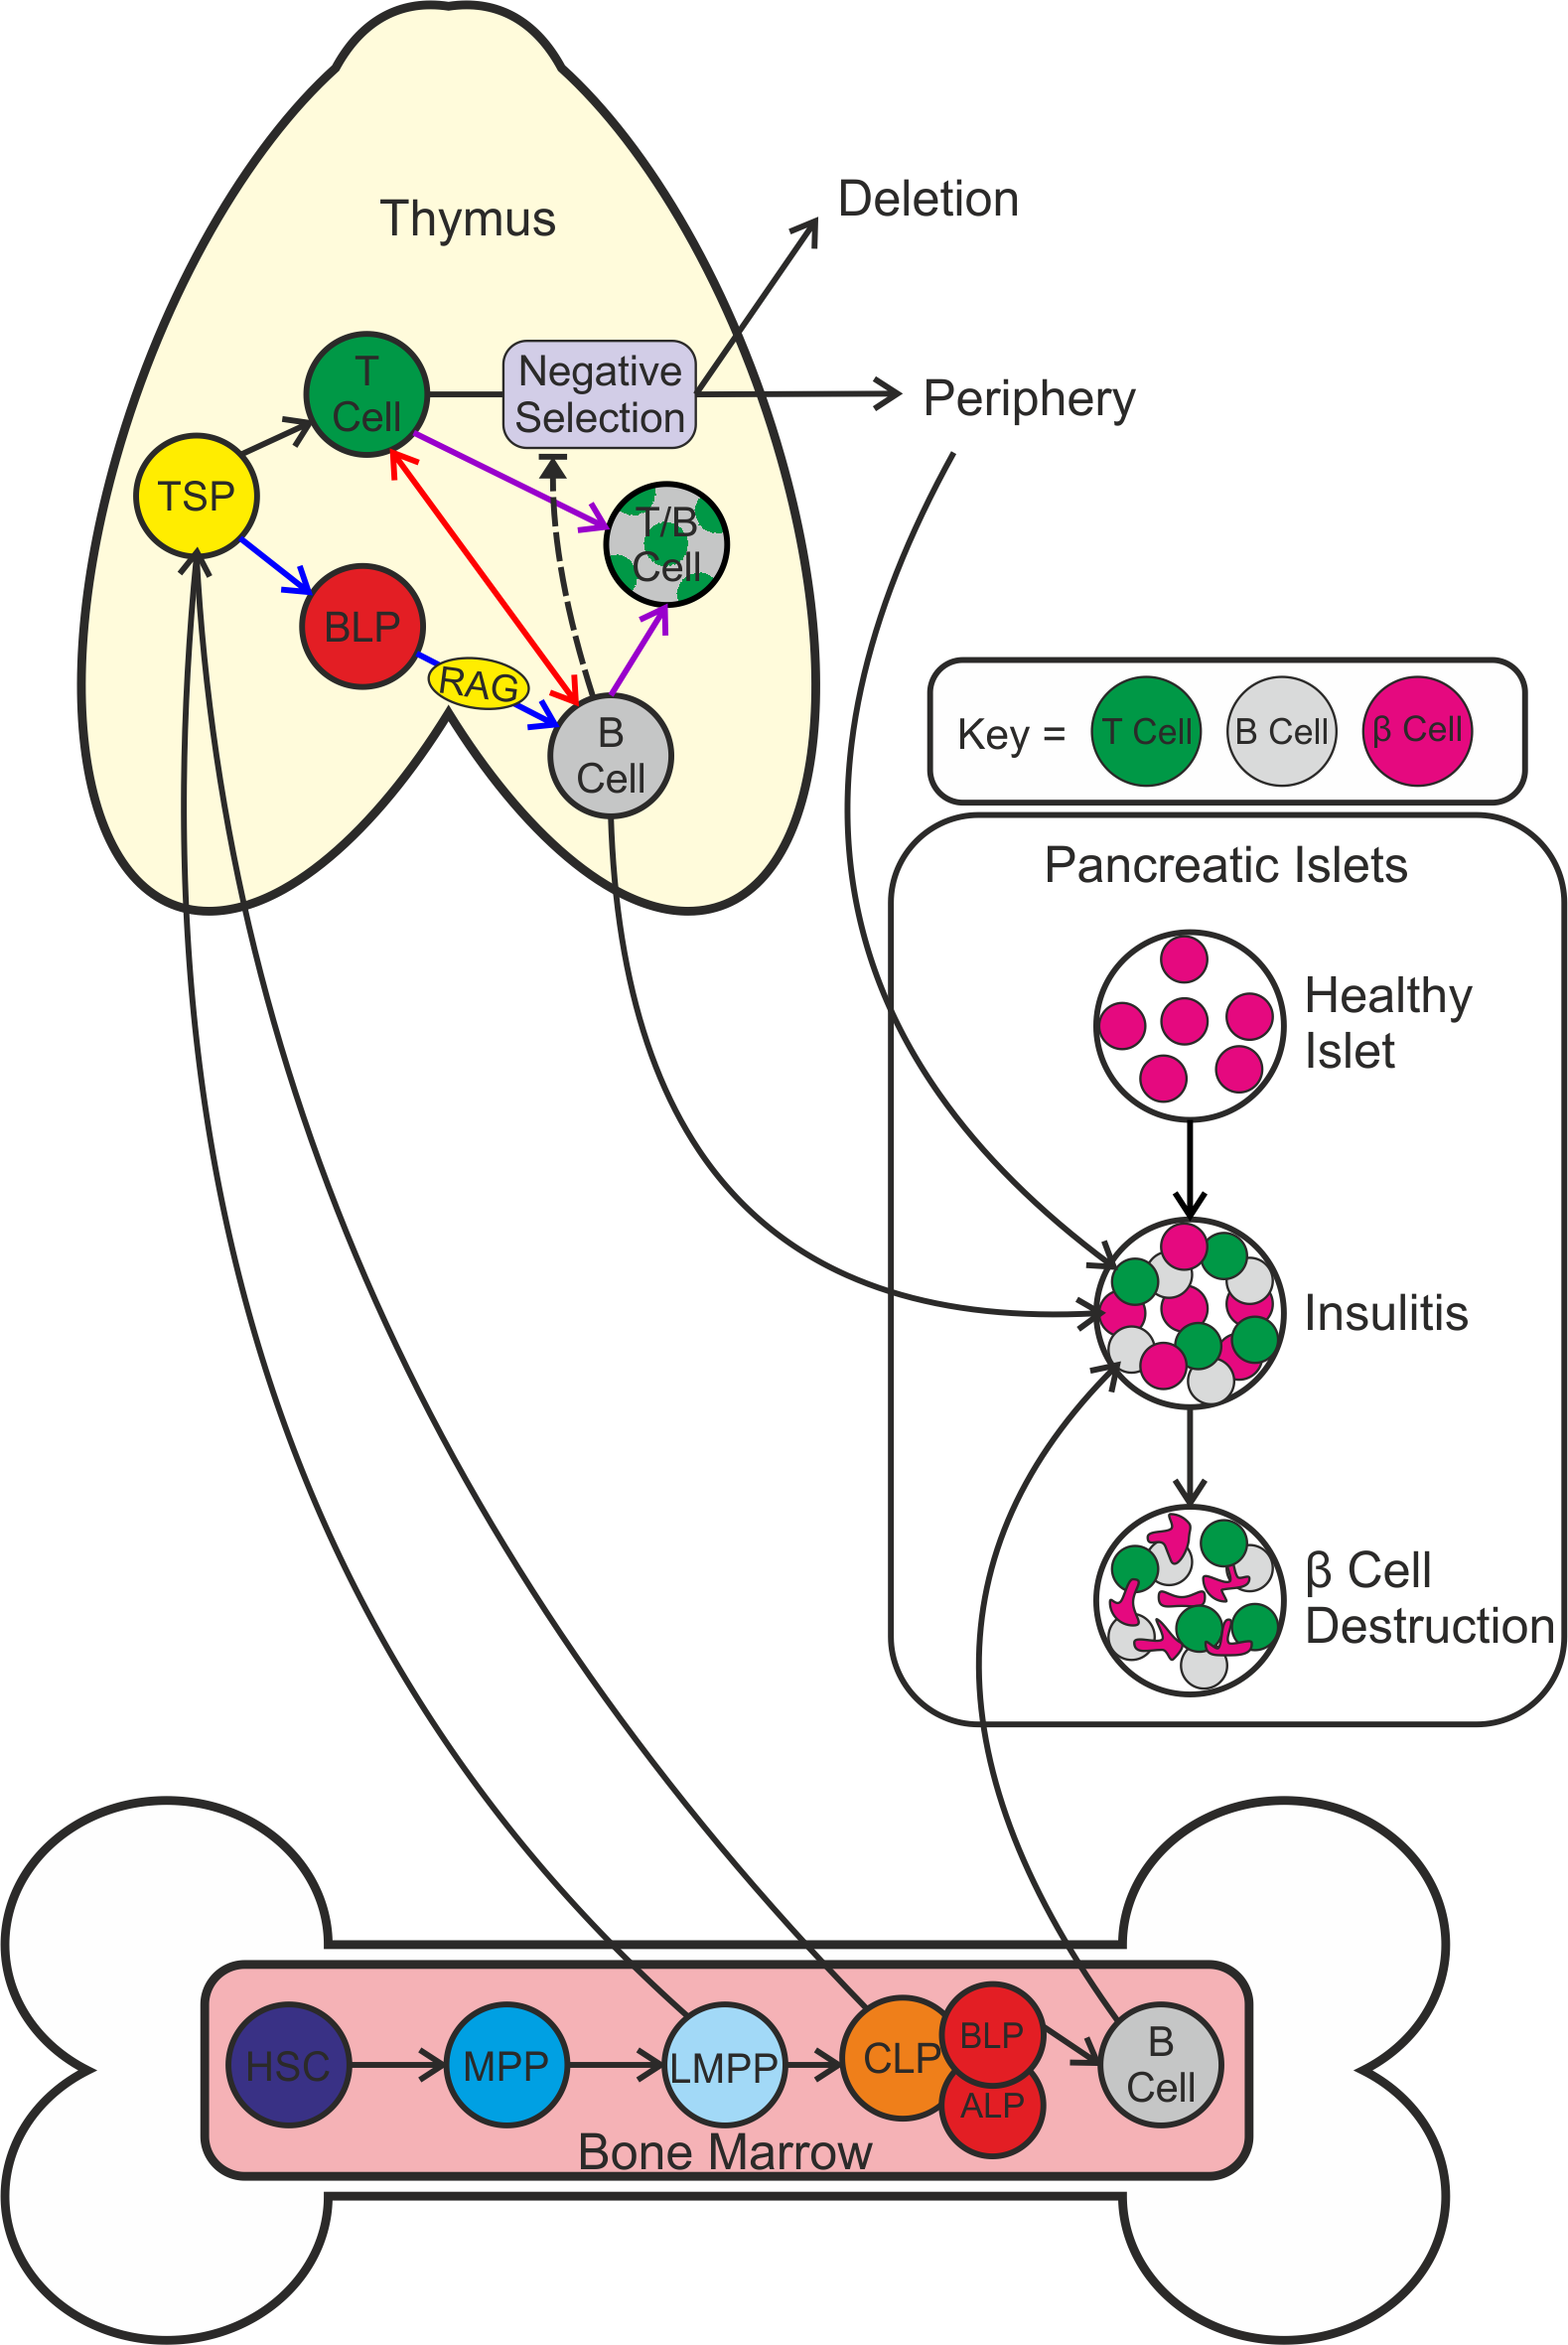
\includegraphics[width=\textwidth]{Figures/diagram2.png}
\caption[Diagrammatical summary of the project findings]{ 
B cells develop in the bone marrow. 
T cells develop from thymic settling progenitors believed to be Flt3\textsuperscript{+}CCR7/9\textsuperscript{+} LMPPs or CLPs which migrate to the thymus.
Here they develop into T cells and pass through negative selection, for which the outcome is either clonal deletion or release into the periphery.
B cells may also be developing in the thymus, either following the same pathway as seen in the bone marrow (bone marrow), or from T cells developing into B cells (red arrows).
There also appears to be evidence of a cell expressing both T and B cell markers which may arise from a B or T cell that has been triggered to display both markers (purple arrows), or may be the mid point of a transitioning T or B cell.
Thymic B cells may contribute to insulitis.}
\label{fig:summarydiagram2}
\end{figure}


By understanding the likely intrathymic development of thymic B cells in the NOD mouse, it may be possible in the future to manipulate this process in order to help with development of therapeutics for T1D.
It would therefore be an obvious progression to look into the functioning of thymic B cells and how their actions have an effect on the T1D pathogenesis.
By linking the development and functioning of thymic B cells, it may be that there is an optimum time point for intervening in the thymic B cell development process in order to have a beneficial effect on the disease.
Not only this but the evidence of thymic B cells also being present in other autoimmune diseases, such as myasthenia gravis, it may be that the knowledge of thymic B cell development and function has far reaching benefits, not just in the context of T1D.












